\chapter{Neues Betriebsmittel anlegen}
\label{Neues Betriebsmittel anlegen}
�ber den Men�punkt Inventar->Neu k�nnen neue Betriebsmittel angelegt werden.
Werden mehrere gleiche Betriebsmittel angelegt, kann eine Vorlage verwendet werden. In diesem Fall m�ssen nur die Daten ge�ndert werden die sich pro Ger�t unterscheiden (etwa Inventarnummer und Seriennummer).\\
Dazu kann in der Auswahlbox im Kopfbereich des Formulares die Anzahl der anzulegenden Betriebsmittel ausgew�hlt werden.
Die eingetragenen Daten werden automatisch f�r die einzelnen Betriebsmittel �bernommen.\\
\\
Die Inventarnummer wird nicht vom System generiert! Diese wird vom Programm des Etikettendruckers erstellt und h�ndisch oder mittels Barcodescanner eingetragen.
Die Details zu den einzlnen Betriebsmitteln k�nnen �ber den Punkt 'Inventardaten anzeigen/ausblenden' angezeigt werden.
Der klick auf einen der 'speichern' Buttons speichert immer alle der angezeigten Betriebsmittel.
\begin{figure}
	\centering
	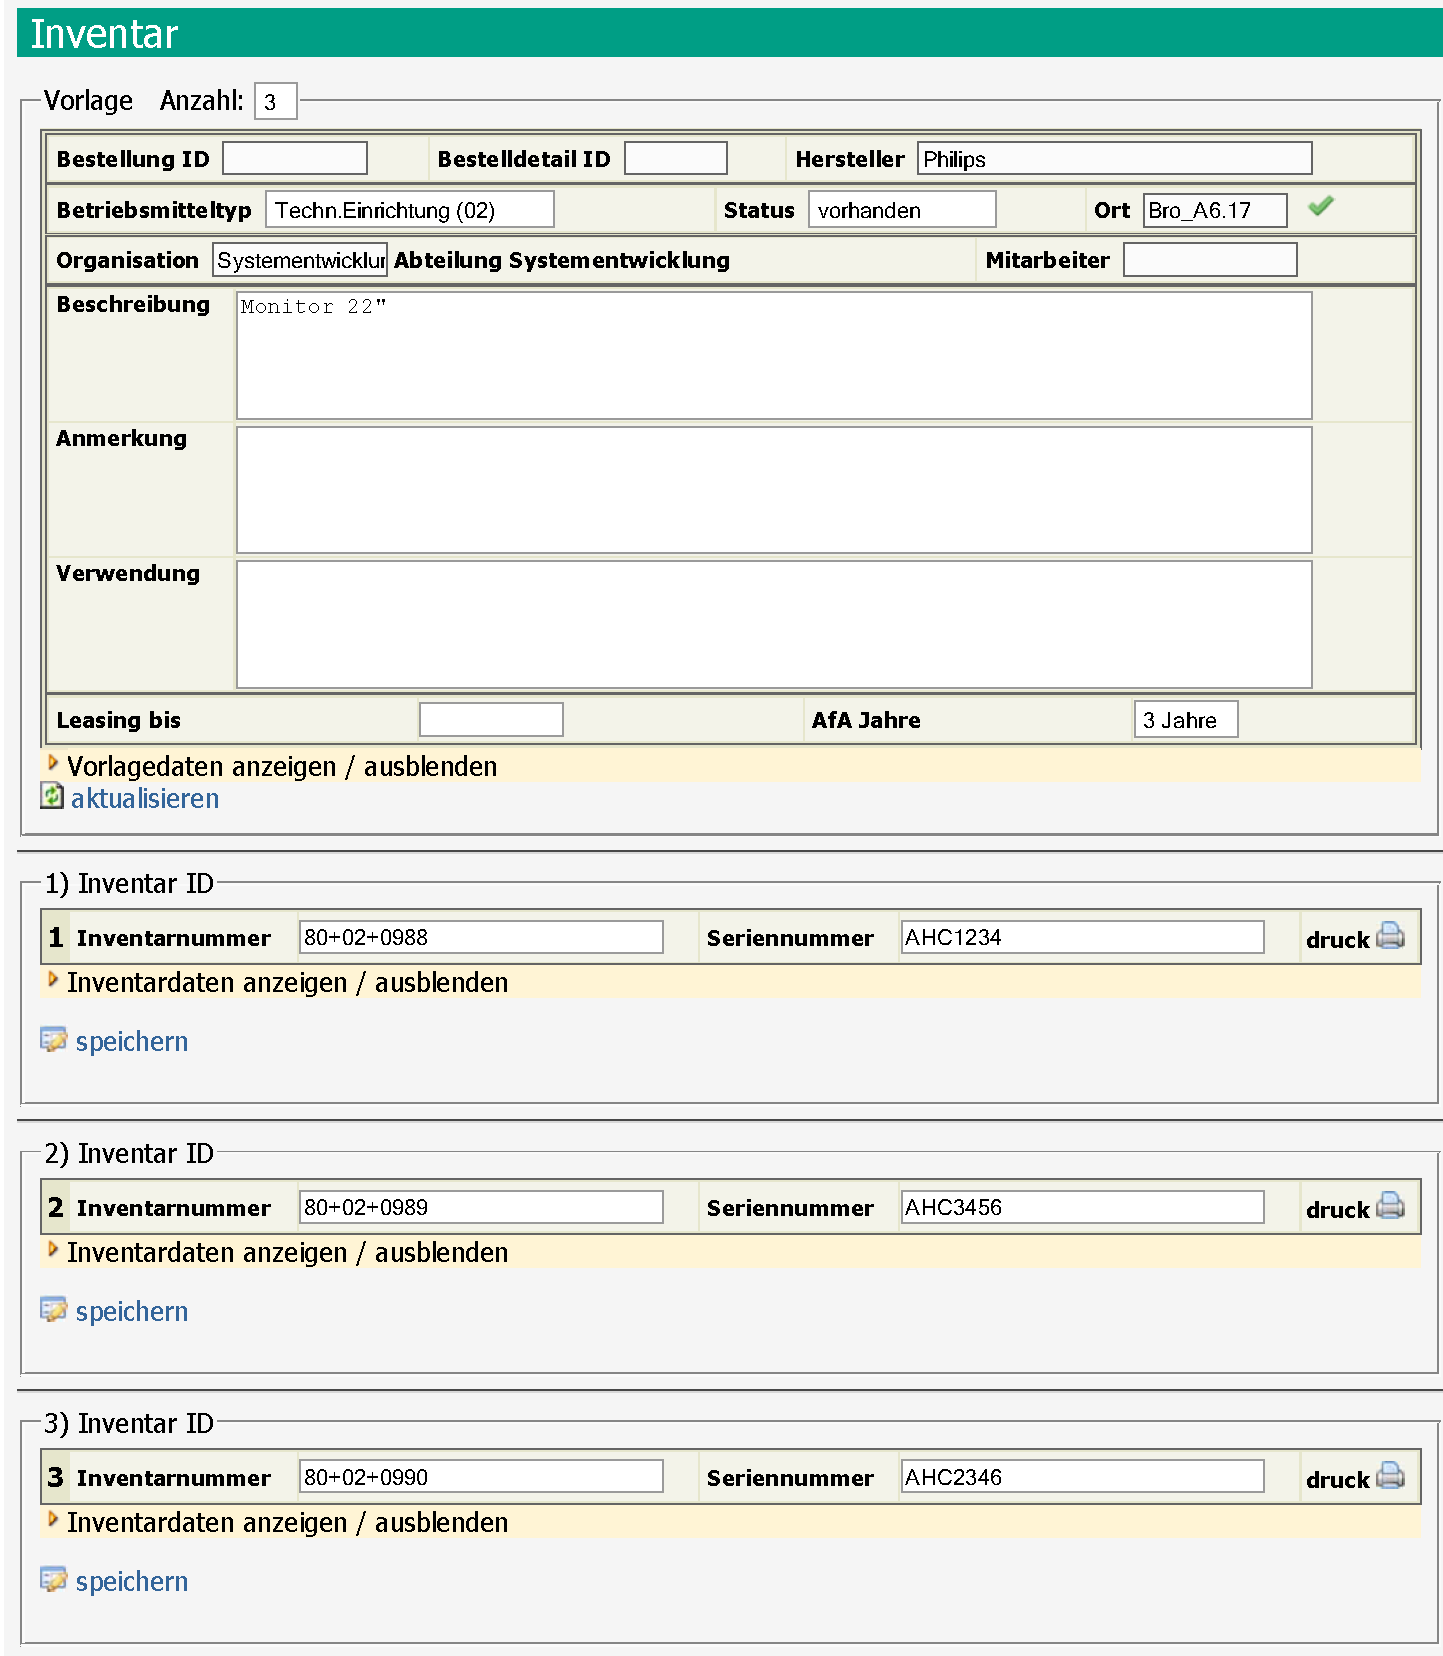
\includegraphics[width=0.80\textwidth]{Inventar_neu.png}
	\caption{Neuanlage}
	\label{Neuanlage}
\end{figure}

